In this section we report our results and findings of static and dynamic instruction count, performance, power, and energy. 

\subsection{Instruction Count}
Figure~\ref{fig:static} shows the static icount obtained from QEMU. As seen in the figure, on average 32bit and 64bit ARM are about 15\% more dense than that of in MIPS and RISCV. Mibench applications have on average 5k instruction that are executed at least once. Figure~\ref{fig:dynamic} shows the dynamic icount obtained from QEMU. Unlike static icount, dynamic icount can be quite different from one application to another for different ISAs. However, on average MIPS, ARM, and RISCV have almost same dynamic icount. 

\begin{figure*}[htb]
	\centering
	%\footnotesize
	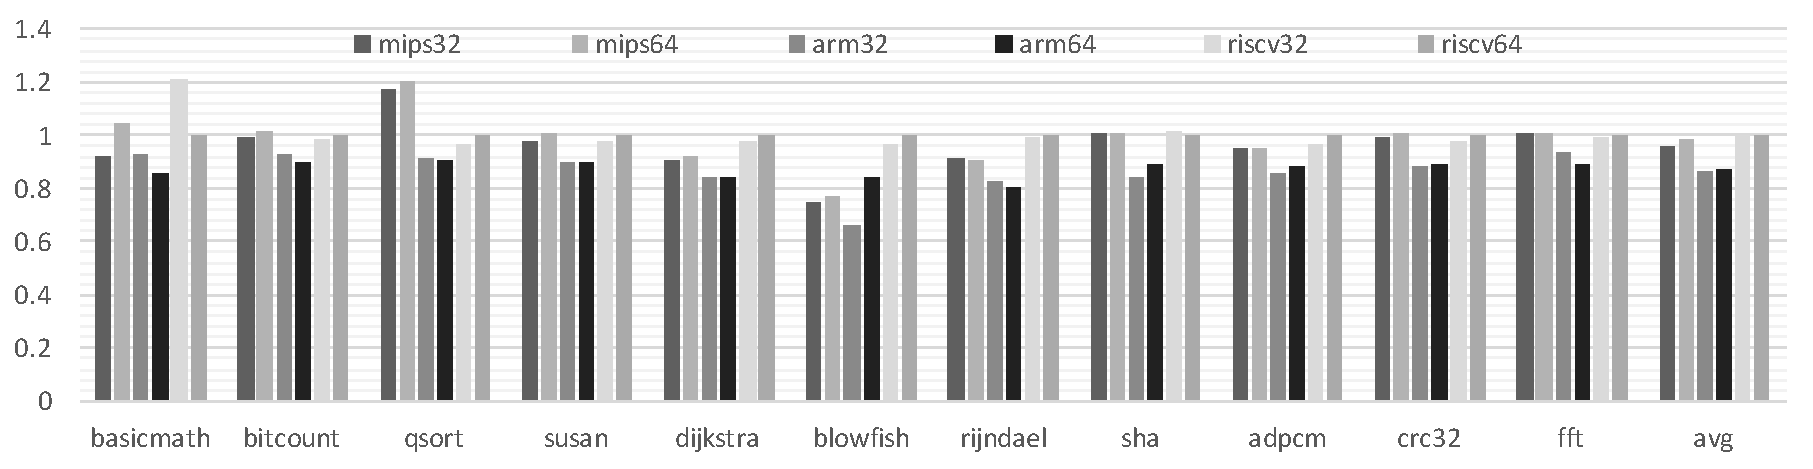
\includegraphics[width=1.8\columnwidth]{figures/static.pdf}
	\caption{Static Instruction Count for MiBench applications using QEMU. Results are normalized w.r.t. RISCV64. The average number of static instructions is about 5000 for these benchmarks.}
	\label{fig:static}
	%\vspace{-1em}
\end{figure*} 

\begin{figure*}[htb]
	\centering
	%\footnotesize
	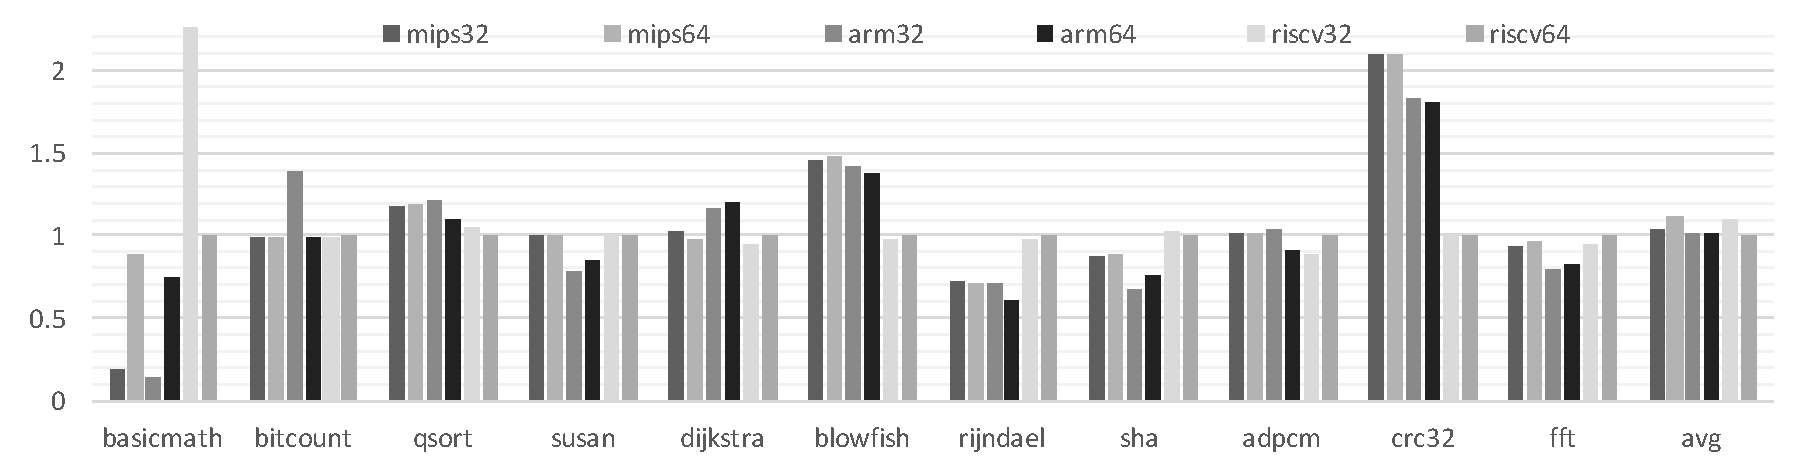
\includegraphics[width=1.8\columnwidth]{figures/dynamic.pdf}
	\caption{Dynamic Instruction Count for MiBench applications using QEMU. Results are normalized w.r.t. RISCV64. The average number of dynamic instructions for these benchmarks is about 450 million.}
	\label{fig:dynamic}
	%\vspace{-1em}
\end{figure*} 

\noindent \textbf{Key Findings}: 1- Mixed/Combined instructions (e.g. add+shift, mult+add, etc.) and three operand/three-way comparison in ARM could result in significant dynamic and static icount reduction. A possible and interesting extension to RISCV could be adding this sort of instructions to the base ISA (RV-G) for high-performance scenarios. An example is shown in Figure~\ref{fig:code}, where a same function is shown for ARM and RISCV ISAs. As seen in this example, ``ldr'' instruction in ARM with embedded ``lsl'' instruction inside it, has saved one instruction. Further ``cmn'' (compare and add), also saved two extra instructions in ARM. We found that there are many examples such as this where more complex instructions in ARM could save more space, however, we will later show that this complexity comes with more power consumption. 

\begin{figure}[t]
	\centering
	%\footnotesize
	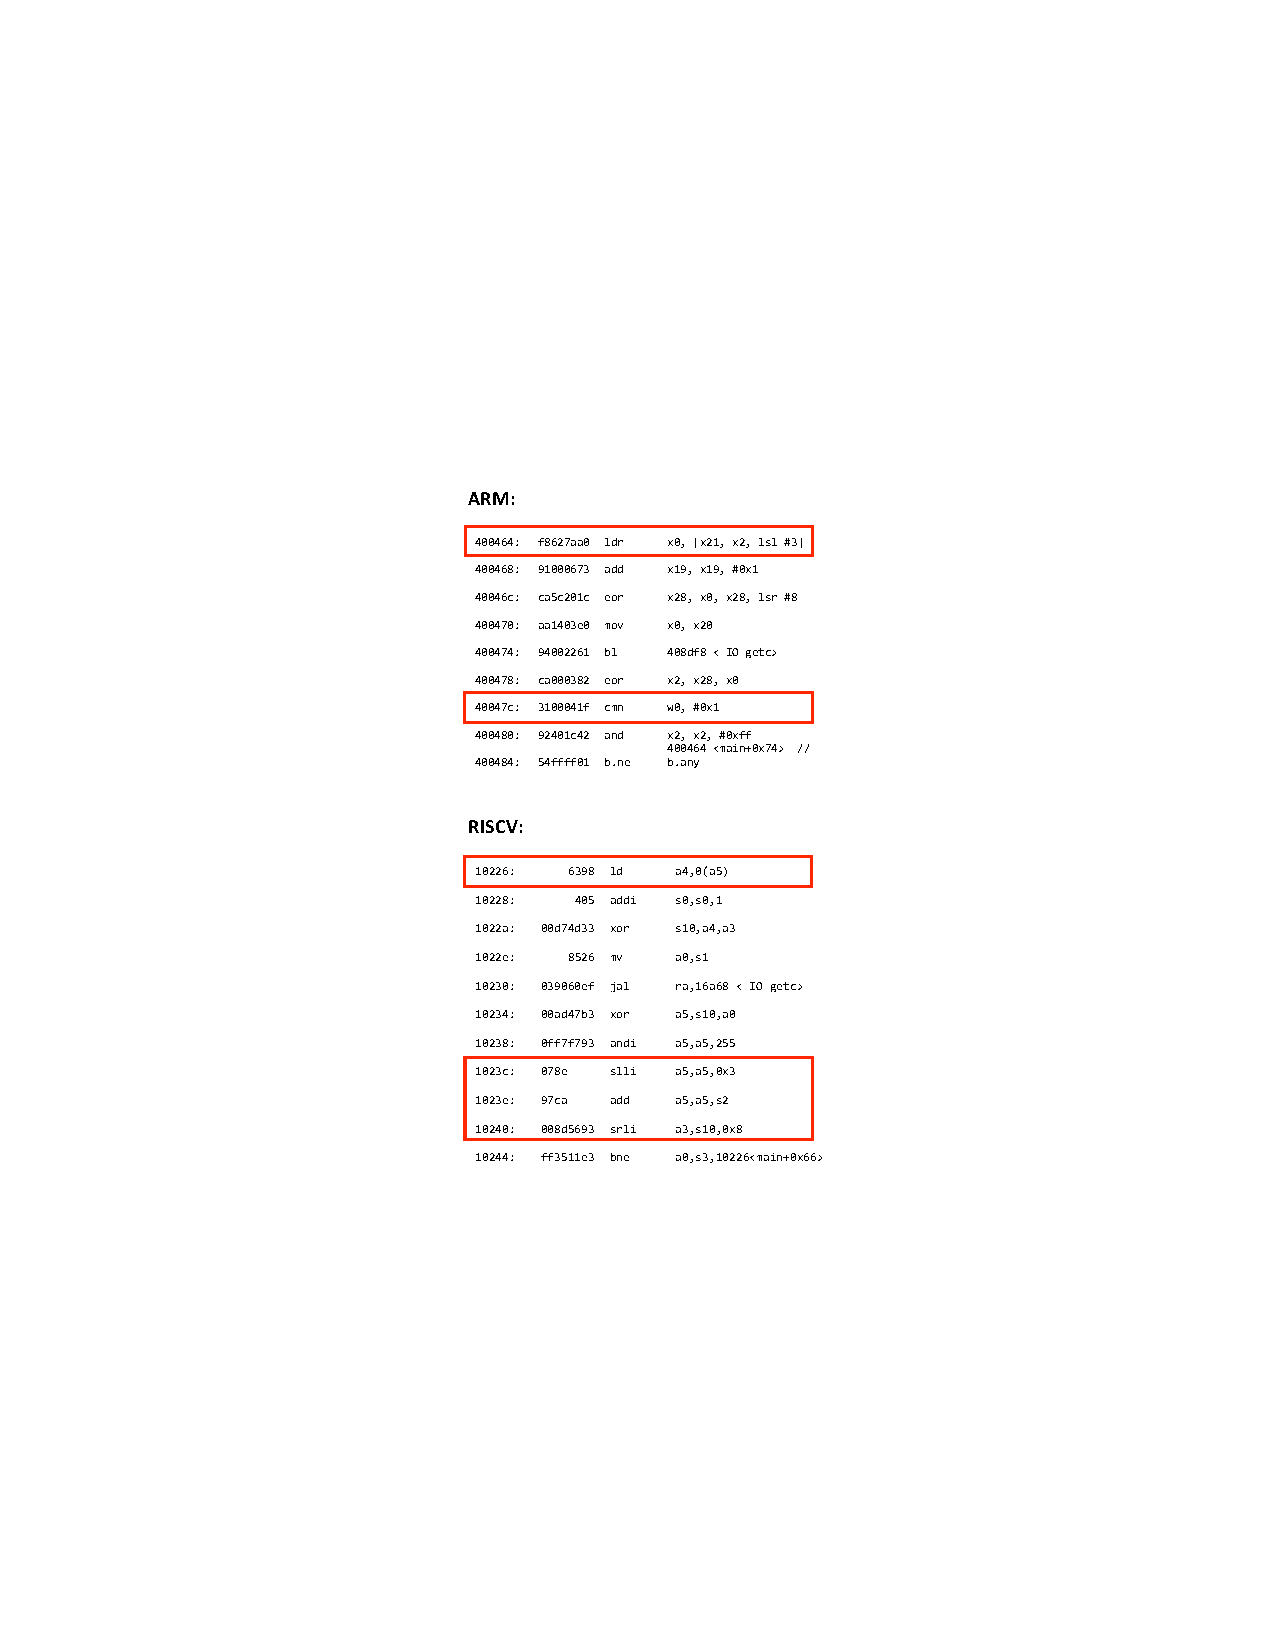
\includegraphics[width=0.9\columnwidth]{figures/code.pdf}
	\caption{A code snippet in assembly showing a same function from Mibench benchmark suite for ARM-64 and RISCV-64 ISAs. Differences shown in rectangles.}
	\label{fig:code}
	%\vspace{-1em}
\end{figure} 

\noindent \textbf{Outliers}: static icount for qsort on MIPS is significantly higher. The main reason for that is due to the way a hot loop in a function called \textsc{msort\_with\_temp} (part of glibc library for quicksort) is implemented in MIPS where a few extra instructions are used for MIPS. Interestingly, we find that this function is implemented slightly different among different toolchains. 
